\section{R\'{e}alisation}
Pour implémenter notre application, nous allons utiliser le moteur Unity\footnote{www.unity3d.com}, un système multiplateforme de création de jeu vidéo développé par Unity Technologies. Ce système comprend un moteur de jeu et un environnement de développement intégré (IDE). L'application sera vu par l'utilisateur à partir d'un casque de réalité virtuelle pour améliorer le sentiment de présence dans le monde virtuel. Pour le casque, nous allons utiliser l'Oculus Rift \cite{oc12} car il s'agit du seul dispositif de ce type disponible sur le lieu de stage.
\subsection{Acquisition des mouvements}
La \emph{Microsoft Kinect} est disponible en deux versions, la première sortie en Novembre 2010 communément appelée \emph{Kinect V1} dont la déclinaison, \emph{Kinect for Windows} qui permet de s'en servir avec un ordinateur, est sortie en Février 2012. La seconde version, \emph{Kinect V2}, est sortie en été 2014. Il existe des différences importantes entre les deux versions, notamment dans le fonctionnement du capteur profondeur \cite{lu15}. En effet, dans la premier version, un motif prédéfini est projeté par rayon infrarouge et la profondeur est calculé en observant les déformations de ce motif. Cependant, comme il existe un espace entre les différents points qui créent le motif, il faut faire une interpolation pour obtenir les valeurs manquantes et le résultat obtenu par le capteur de profondeur peut manquer de précision. Pour la seconde version, \emph{Microsoft} a utilisé une technologie différente basée sur le temps de vol. Des rayons infrarouges sont envoyés dans la zone vue par la \emph{Kinect v2} et la réflexion des rayons est détectée par le capteur de profondeur. \`{A} partir du temps écoulé entre ces deux événements, la profondeur peut être calculée pour chaque pixels qui composent l'image obtenu. Les utilisateurs face à la \emph{Kinect} sont détectés et suivis à partir de l'image obtenu par le capteur de profondeur qui est ensuite traitée pour reconnaitre les formes humaines, ce qui fait que la \emph{Kinect V2} permet une meilleure capture des mouvements que la version précédente. De plus, la version récente capture plus de points sur la personne suivie que la première version, 25 pour la \emph{Kinect V2}(Voir Figure \ref{track}) et 20 pour la \emph{Kinect V1}, nous allons donc, pour capturer les mouvements de l'utilisateur, utiliser la seconde version de la \emph{Microsoft Kinect}.\\

\begin{figure}[!h]
   	\centerline{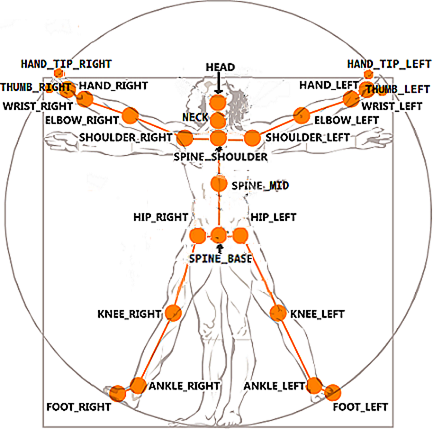
\includegraphics[scale=0.7]{images/kinectTracking}}
   	\caption{\label{track} 25 points reconnus par la \emph{Kinect V2} }
\end{figure}

La \emph{Microsoft Kinect V2} permet d'obtenir la position et l'orientation de chacun des 25 points reconnus sur l'utilisateur. Pour contrôler l'avatar, il n'est pas possible d'utiliser la position des points obtenus car elle dépends en partie de la morphologie de la personne dont les mouvements sont capturés. Cela modifierait la longueur des différents membres de l'avatar et aurait donc un impact négatif sur son apparence. On utilise donc l'orientation des points pour modifier la rotation au niveau des différentes articulations de l'avatar. Pour s'assurer que les valeurs obtenus par la \emph{Kinect} ne sont pas irréaliste, les valeurs sont filtrées pour respecter les rotations permises par les articulation du corps humain.\\

Pour obtenir les mouvements du bâton virtuel, nous utilisons une des deux manettes de la \emph{Razer Hydra}  (Voir Figure \ref{Razer}) à laquelle nous accrochons directement le bâton réel qui servira à toucher l'utilisateur dans le dos. De cette façon, nous pouvons récupérer la position et l'inclinaison de la manette dans un espace en trois dimensions par rapport à la base de la \emph{Razer Hydra}, ce qui correspond également à ceux du bâton. L'appareil étant fait pour le jeu, chacune des manettes possèdent six boutons et un joystick qui nous servent à déplacer le bâton virtuel afin de s'assurer au début de l'application que la position du bâton virtuel correspond bien à celui du bâton réel avant de commencer à toucher la personne dans le dos (Voir Figure \ref{batonAvatar}). Comme la \emph{Razer Hydra} donne la position et l'inclinaison, on peut déplacer le bâton virtuel pour qu'il reproduise les mouvements du bâton réel en obtenant un résultat fluide et fidèle.
\begin{figure}[!h]
   	\centerline{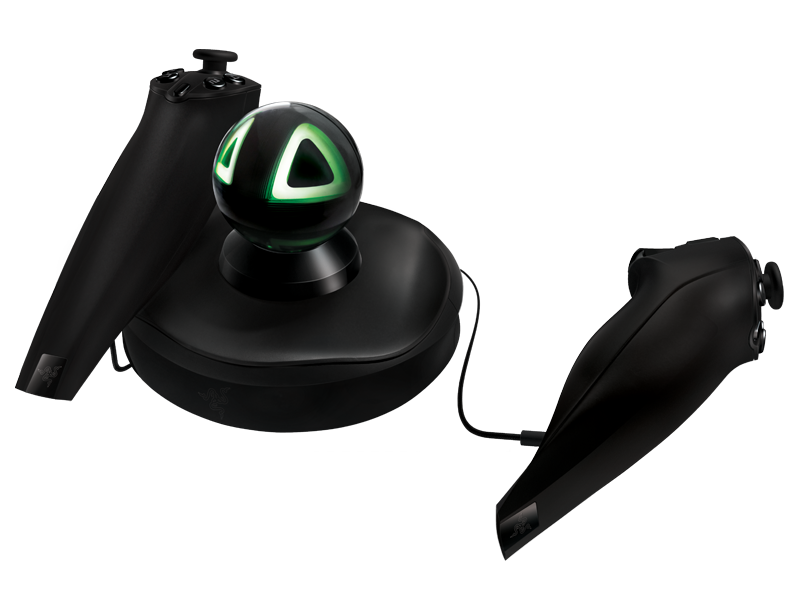
\includegraphics[scale=0.2]{images/biblio/razerHydra}}
  	\caption{\label{Razer} \emph{Razer Hydra}}
\end{figure}
\begin{figure}[!h]
   	\centerline{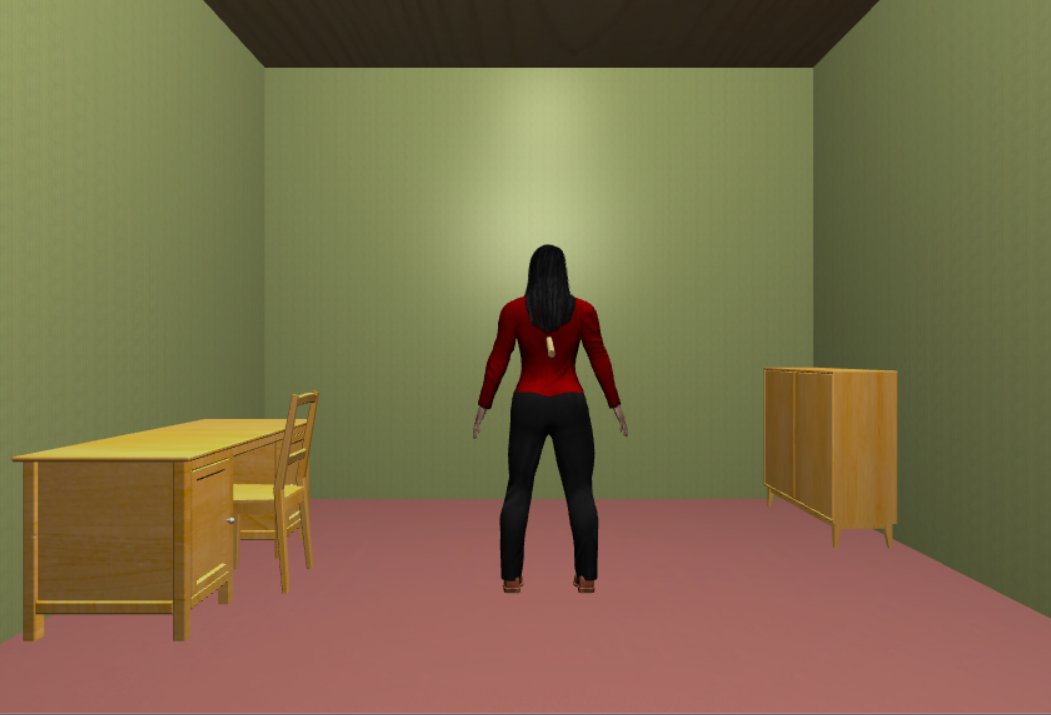
\includegraphics[scale=0.5]{images/avatarBaton2}}
   	\caption{\label{batonAvatar} Avatar touché par le bâton virtuel }
\end{figure}
\subsection{Avatars}
\subsubsection{Création et choix des modèles}
Comme précisé dans la section précédente, nous utilisons \emph{MakeHuman} pour créer nos modèles de personnage. Pour créer de nombreux modèles avec des corpulences différentes, nous avons utilisé deux des paramètres proposé par ce logiciel pour modifier l'apparence : la masse et le muscle. La masse permet donc de modifier le poids de l'avatar et le paramètre muscle permet de changer la musculation de l'avatar. Ces deux paramètres prennent des valeurs entre 0\% et 100\%. On crée ainsi des modèles qui ont 0\%, 25\%, 50\%, 75\% et 100\% de masse et pour chacune de ces valeurs, on prend des valeurs de musculation de 0\%, 25\%, 50\%, 75\% et 100\%. Ce qui nous donne vingt-cinq modèles différents. \emph{MakeHuman} permet de faire des personnages femme et homme et nous créons donc des avatars des deux genres pour convenir à la fois à un utilisateur et une utilisatrice. Lors du lancement de l'application, l'utilisateur est d'abord invité à choisir son avatar parmi les vingt-cinq proposés. Les avatars proposés par l'interface varie en fonction du genre de l'utilisateur (Voir Figure \ref{uiF}). L'utilisateur peut alors sélectionner l'avatar lui ressemblant le plus selon lui en cochant la \emph{checkbox} associée au modèle. L'expérimentateur peut ensuite choisir un autre avatar qui correspond plus à la véritable apparence de l'utilisateur.
\begin{figure}[!h]
   	\centerline{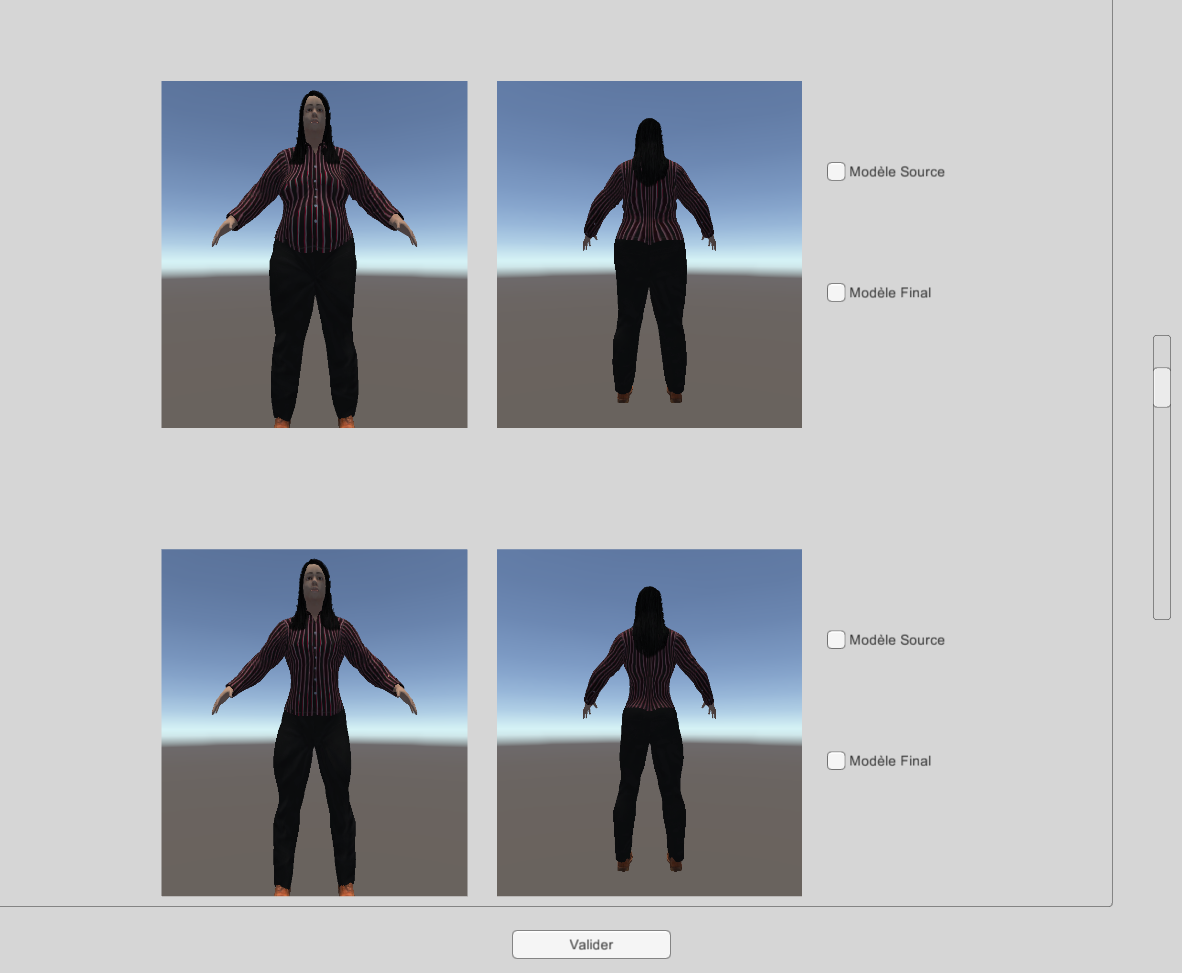
\includegraphics[scale=0.30]{images/interfaceF}}
   	\caption{\label{uiF} Interface pour choisir un avatar féminin }
\end{figure}
\subsubsection{Modification de l'avatar}
Comme nos avatars sont tous créés grâce à \emph{MakeHuman}, nous pouvons nous assurer que chacun de nos modèles est définit de la même manière, le maillage du personnage (\emph{Mesh}) est définit avec le même nombre de point (\emph{Vertex}), ce qui nous permet d'utiliser le \emph{Morphing 3D}, une technique demandant peu de calcul et donc bien adaptée au temps réel. Durant notre modification, seul la forme de l'avatar change, c'est-à-dire que seul le maillage, qui permet de créer la forme du modèle, est modifié. Les textures restent les mêmes durant la modification. Le \emph{Morphing 3D} est réalisé via un calcul d'interpolation linéaire. Pour cela on calcule chaque point intermédiaire de cette façon :
\begin{center}
$P = \alpha*P_i + (1-\alpha)*P_j$, avec $0<\alpha<1$
\end{center}
Avec $P$ qui est le point intermédiaire, $P_i$ et $P_j$ sont les points équivalents appartenant respectivement au modèle de départ et au modèle d'arrivé. Avec le moteur, nous avons défini que le calcul serait réalisé toute les 20ms. Nous souhaitons que la modification se fasse sur la durée d'une minute, ce qui fait que lors de notre \emph{Morphing 3D}, un total de 3000 modèles intermédiaires sont calculés et vus par l'utilisateur. Le but qu'on cherche à atteindre avec ce paramétrage et ce nombre de modèle intermédiaire calculé, est d'obtenir une modification suffisamment subtile pour que l'utilisateur ne se rende pas tout de suite compte que son avatar est en train de changer mais plutôt qu'il se rende compte après la modification ou vers la fin que son avatar a changé. Sur la Figure \ref{morphingGhost}, on peut voir un avatar après avoir été modifié et en transparent apparait la forme d'origine.

\begin{figure}[!h]
   	\centerline{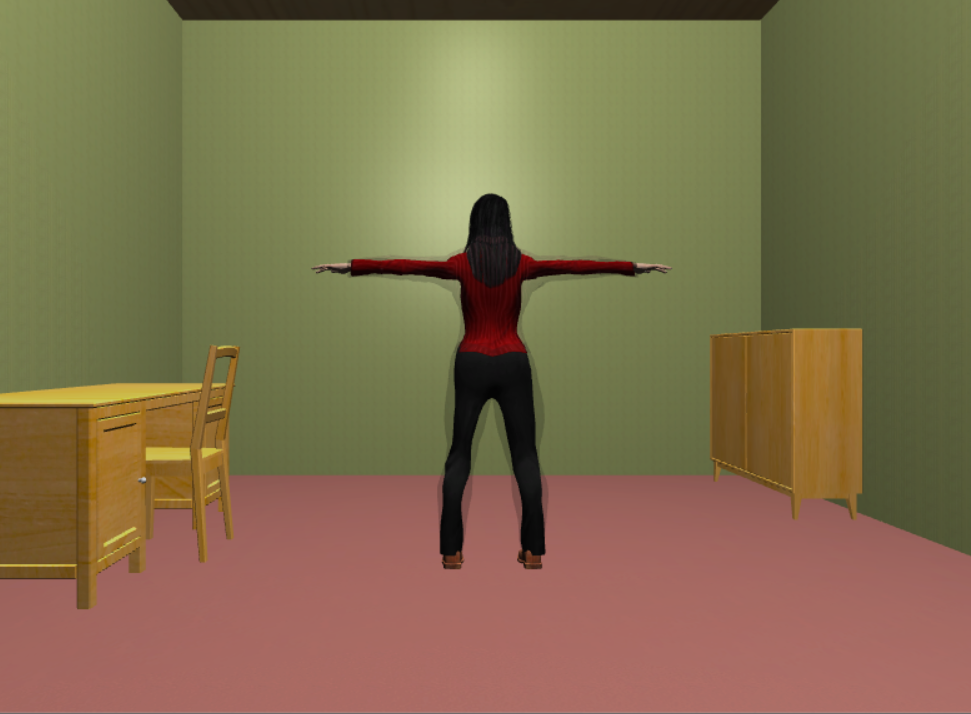
\includegraphics[scale=0.5]{images/morphingGhost2}}
   	\caption{\label{morphingGhost} Modèle après modification avec apparence d'origine en transparence }
\end{figure}
